\chapter{Fit for $F_{+}$}

\section{Fractional flavour-tagged \KsPiPi yields $T_i$}
The given values for $K'_i$ obtained from Table 1 of \texttt{arXiv:1210.939} contain effects from charm-mixing that cancel in our case. The factors $T_i$ without mixing are archived by numerically solving the system of equations:
\begin{equation}
K'_i = T_i + \sqrt{T_i T_{-i}} (y c_i + x s_i)
\end{equation}
where $x$ and $y$ charm-mixing parameters. The fit also takes into account that the sum over the $T_i$ should be one by fixing  $T_1 = 1 - \sum_{i \neq 1} T_i$. The values for $x$ and $y$ are take from the latest HFAG results ($x = (0.63 \pm 0.19)\%$, $y = (0.75 \pm 0.12)\% $) and the values for $c_i$ and $s_i$ are taken from \texttt{arXiv:1010.2817}. In the fit all input variables are Gaussian constraint and the correlation between $c_i$ and $s_i$ are taken into account. The resulting $T_i$ are listed below.\\
\begin{table}[!h]
	\begin{center}
		\begin{tabular}{c| c | c |c }
			bin & $T_i$ & bin & $T_i$ \\
			\hline
			1 & 0.1695 $\pm $ 0.0053 \qquad & -1 & 0.0781 $\pm$ 0.0014 \\
			2 & 0.0873 $\pm $ 0.0012 \qquad & -2 & 0.0186 $\pm$ 0.0002 \\
			3 & 0.0723 $\pm $ 0.0020 \qquad & -3 & 0.0201 $\pm$ 0.0003 \\
			4 & 0.0258 $\pm $ 0.0011 \qquad & -4 & 0.0161 $\pm$ 0.0015 \\
			5 & 0.0889 $\pm $ 0.0024 \qquad & -5 & 0.0523 $\pm$ 0.0013 \\
			6 & 0.0589 $\pm $ 0.0011 \qquad & -6 & 0.0147 $\pm$ 0.0003 \\
			7 & 0.1252 $\pm $ 0.0018 \qquad & -7 & 0.0132 $\pm$ 0.0004 \\
			8 & 0.1320 $\pm $ 0.0021 \qquad & -8 & 0.0270 $\pm$ 0.0010 \\
			\end{tabular}
\end{center}
\caption{\textit{Fraction flavour-tagged \KsPiPi yields without mixing-effects.}}
\end{table} 
\clearpage
\section{Fractional flavour-tagged \KlPiPi yields $T'_i$}
The fractional flavour-tagged \KlPiPi yields are taken from Sean Brisbane's thesis (Section 3., Table 3.14). They are listed below:
\begin{table}[!h]
	\begin{center}
		\begin{tabular}{c| c | c |c }
			bin & $T'_i$ & bin & $T'_i$ \\
			\hline
1 & 0.163 $ \pm $ 0.004 \qquad & -1 & 0.090 $ \pm $ 0.017 \\ 
2 & 0.069 $ \pm $ 0.003 \qquad & -2 & 0.024 $ \pm $ 0.005 \\ 
3 & 0.061 $ \pm $ 0.003 \qquad & -3 & 0.031 $ \pm $ 0.006 \\ 
4 & 0.026 $ \pm $ 0.002 \qquad & -4 & 0.019 $ \pm $ 0.004 \\ 
5 & 0.082 $ \pm $ 0.003 \qquad & -5 & 0.057 $ \pm $ 0.014 \\ 
6 & 0.058 $ \pm $ 0.002 \qquad & -6 & 0.017 $ \pm $ 0.004 \\ 
7 & 0.122 $ \pm $ 0.003 \qquad & -7 & 0.021 $ \pm $ 0.003 \\ 
8 & 0.124 $ \pm $ 0.003 \qquad & -8 & 0.035 $ \pm $ 0.008 \\ 


\end{tabular}
\end{center}
\caption{\textit{Fraction flavour-tagged \KlPiPi yields.}}
\end{table} 


\section{Results $F_+$ }
A fit for $F_+$ is performed for the default signal results, for the results with stat. error only, and for each systematic effect listed in Chapter \ref{c:sys}. The error from the systematic error from the signal selection and reconstruction efficiency and the limited data and MC sample used to determine the peaking bkg distributions (those were determined alongside the statistical error) are determined by comparing the fit results with stat. error only and stat. error $\oplus$ sys. error.
\begin{table}[!h]
\begin{center}
\begin{tabular}{c| c | c| c}
 & \KsPiPi Fit & \KlPiPi Fit & sim. Fit\\
 \hline
\multirow{4}{*}{default} & $\mathbf F^{\KsPiPi}_{+}$\textbf{ = 0.8279} $\mathbf \pm$ \textbf{0.0750} & $\mathbf F^{\KlPiPi}_{+}$\textbf{ = 0.6700} $\mathbf \pm$ \textbf{0.0639} & $\mathbf F^{sim}_{+}$ \textbf{= 0.7372} $\mathbf \pm$ \textbf{0.0510} \\
& $h^{\KsPiPi}_{norm}$ = 111.9 $\pm$ 8.88 &  & $h^{\KsPiPi}_{norm}$ = 110.49 $\pm$ 8.83 \\
& &  $h^{\KlPiPi}_{norm}$ =  220.19 $\pm$ 15.01 & $h^{\KlPiPi}_{norm}$ = 213.11 $\pm$ 14.41 \\
 &  $\chi^2_{ndof}$ = 0.64 &  $\chi^2_{ndof}$ = 0.72 &  $\chi^2_{ndof}$ = 0.403 \\
\hline 
\hline
\multirow{4}{*}{stat. only} & $F^{\KsPiPi}_{+}$ = 0.8279 $\pm$ 0.0746 & $F^{\KlPiPi}_{+}$ = 0.6701 $\pm$ 0.0637 & $F^{sim}_{+}$ = 0.7374 $\pm$ 0.0508 \\
& $h^{\KsPiPi}_{norm}$ = 111.9 $\pm$ 8.82 &  & $h^{\KsPiPi}_{norm}$ = 110.48 $\pm$ 8.78 \\
& &  $h^{\KlPiPi}_{norm}$ =  220.14 $\pm$ 14.95 & $h^{\KlPiPi}_{norm}$ = 213.11 $\pm$ 14.35 \\
 &  $\chi^2_{ndof}$ = 0.64 &  $\chi^2_{ndof}$ = 0.72 &  $\chi^2_{ndof}$ = 0.407 \\
\hline 
\hline
\multirow{4}{*}{flat bkg} & $F^{\KsPiPi}_{+}$ = 0.8230 $\pm$ 0.0727 & $F^{\KlPiPi}_{+}$ = 0.6445 $\pm$ 0.0606 & $F^{sim}_{+}$ = 0.7173 $\pm$ 0.0488 \\
& $h^{\KsPiPi}_{norm}$ = 112.01 $\pm$ 8.69 &  & $h^{\KsPiPi}_{norm}$ = 110.75 $\pm$ 8.64 \\
& &  $h^{\KlPiPi}_{norm}$ =  218.19 $\pm$ 14.40 & $h^{\KlPiPi}_{norm}$ = 212.36 $\pm$ 13.84 \\
 &  $\chi^2_{ndof}$ = 0.61 &  $\chi^2_{ndof}$ = 1.11 &  $\chi^2_{ndof}$ = 0.438 \\

\hline 
\hline
\multirow{2}{*}{peak} & $F^{\KsPiPi}_{+}$ = 0.8287 $\pm$ 0.0749 & $F^{\KlPiPi}_{+}$ = 0.6697 $\pm$ 0.0639 & $F^{sim}_{+}$ = 0.7375 $\pm$ 0.0510 \\
& $h^{\KsPiPi}_{norm}$ = 111.87 $\pm$ 8.83 &  & $h^{\KsPiPi}_{norm}$ = 110.49 $\pm$ 8.78 \\
\multirow{2}{*}{clean.} & &  $h^{\KlPiPi}_{norm}$ =  220.24 $\pm$ 15.01 & $h^{\KlPiPi}_{norm}$ = 213.08 $\pm$ 14.41 \\
 &  $\chi^2_{ndof}$ = 0.63 &  $\chi^2_{ndof}$ = 0.72 &  $\chi^2_{ndof}$ = 0.402 \\
\hline 
\hline
\multirow{1}{*}{0.8} & $F^{\KsPiPi}_{+}$ = 0.8279 $\pm$ 0.0750 & $F^{\KlPiPi}_{+}$ = 0.6694 $\pm$ 0.0629 & $F^{sim}_{+}$ = 0.7356 $\pm$ 0.0505 \\
\multirow{1}{*}{BR_{\KlPiPi}}& $h^{\KsPiPi}_{norm}$ = 111.9 $\pm$ 8.88 &  & $h^{\KsPiPi}_{norm}$ = 110.44 $\pm$ 8.83 \\
\multirow{2}{*}{\ref{s:peakc}} & &  $h^{\KlPiPi}_{norm}$ =  223.55 $\pm$ 14.99 & $h^{\KlPiPi}_{norm}$ = 216.53 $\pm$ 14.41 \\
 &  $\chi^2_{ndof}$ = 0.64 &  $\chi^2_{ndof}$ = 0.73 &  $\chi^2_{ndof}$ = 0.407 \\
\hline 
\hline
\multirow{1}{*}{1.2} & $F^{\KsPiPi}_{+}$ = 0.8279 $\pm$ 0.0750 & $F^{\KlPiPi}_{+}$ = 0.6706 $\pm$ 0.065 & $F^{sim}_{+}$ = 0.7396 $\pm$ 0.0520 \\
\multirow{1}{*}{BR_{\KlPiPi}}& $h^{\KsPiPi}_{norm}$ = 111.9 $\pm$ 8.88 &  & $h^{\KsPiPi}_{norm}$ = 110.55 $\pm$ 8.83 \\
\multirow{2}{*}{\ref{s:peakc}} & &  $h^{\KlPiPi}_{norm}$ =  216.81 $\pm$ 15.03 & $h^{\KlPiPi}_{norm}$ = 209.67 $\pm$ 14.41 \\
 &  $\chi^2_{ndof}$ = 0.64 &  $\chi^2_{ndof}$ = 0.71 &  $\chi^2_{ndof}$ = 0.397 \\

\hline 
\hline
\multirow{1}{*}{mult.} & F^{\KsPiPi}_{+} = 0.8351 $\pm$ 0.0777 & F^{\KlPiPi}_{+} = 0.6751 $\pm$ 0.0640 & F^{sim}_{+} = 0.7406 $\pm$ 0.0516 \\
\multirow{1}{*}{cand.} & h^{\KsPiPi}_{norm} = 110 $\pm$ 8.96 &  & h^{\KsPiPi}_{norm} = 108.84 $\pm$ 8.93 \\
\multirow{2}{*}{sel.} & &  h^{\KlPiPi}_{norm} =  220.11 $\pm$ 15.00 & h^{\KlPiPi}_{norm} = 213.32 $\pm$ 14.45 \\
 &  $\chi^2_{ndof}$ = 0.41 &  $\chi^2_{ndof}$ = 0.59 &  $\chi^2_{ndof}$ = 0.298 \\
\hline 
\hline
\multirow{2}{*}{Dalitz} & $F^{\KsPiPi}_{+}$ = 0.8305 $\pm$ 0.0786 & $F^{\KlPiPi}_{+}$ = 0.6692 $\pm$ 0.0644 & $F^{sim}_{+}$ = 0.7349 $\pm$ 0.0522 \\
& $h^{\KsPiPi}_{norm}$ = 108.77 $\pm$ 9.05 &  & $h^{\KsPiPi}_{norm}$ = 107.44 $\pm$ 9.00 \\
\multirow{2}{*}{accept.} & &  $h^{\KlPiPi}_{norm}$ =  221.53 $\pm$ 15.30 & $h^{\KlPiPi}_{norm}$ = 214.58 $\pm$ 14.75 \\
 &  $\chi^2_{ndof}$ = 0.92 &  $\chi^2_{ndof}$ = 0.72 &  $\chi^2_{ndof}$ = 0.538 \\
\hline 
\hline
\multirow{2}{*}{$c_i$ etc.} & $F^{\KsPiPi}_{+}$ = 0.8277 $\pm$ 0.0743 & $F^{\KlPiPi}_{+}$ = 0.6660 $\pm$ 0.0572 & $F^{sim}_{+}$ = 0.7289 $\pm$ 0.0494 \\
& $h^{\KsPiPi}_{norm}$ = 111.77 $\pm$ 8.69 &  & $h^{\KsPiPi}_{norm}$ = 110.05 $\pm$ 8.71 \\
\multirow{2}{*}{fixed}& &  $h^{\KlPiPi}_{norm}$ =  220.18 $\pm$ 13.75 & $h^{\KlPiPi}_{norm}$ = 212.5 $\pm$ 13.44 \\
 &  $\chi^2_{ndof}$ = 0.65 &  $\chi^2_{ndof}$ = 0.91 &  $\chi^2_{ndof}$ = 0.434 \\
\end{tabular}
\end{center}
\caption{\textit{Fit results for the default signal yields and the signal yields with systematic effects.}}
\end{table} 


\begin{table}[!h]
\begin{center}
\begin{tabular}{l| c }
source & uncertainty\\
\hline
\hline
stat. error & $\pm$ 0.0508 \\
\hline
sys. error & $\pm$ 0.0045 \\
\hline
non-flat bkg & $\pm$ 0.0199 \\
\hline
peak bkg clean. & $\pm$ 0.0003 \\
\hline
diff. BR(\KlPiPi) & $\pm$^{0.0024}_{0.0016} \approx $\pm$ 0.002\\
\hline
mult. cand. sel. & $\pm$ 0.0034 \\
\hline
Dalitz acceptance & $\pm$ 0.0023\\
\end{tabular}
\end{center}
\caption{\textit{Uncertainties on the value of $F_+$ from different sources.}}
\end{table} 

Listing the statistical error and the systematic error from the Dalitz plot acceptance separately this results in $F_+ = 0.7372 \pm 0.0508 \pm 0.0208 \pm 0.0023$.

\begin{figure}[!h]
\begin{center}
\subfigure{ 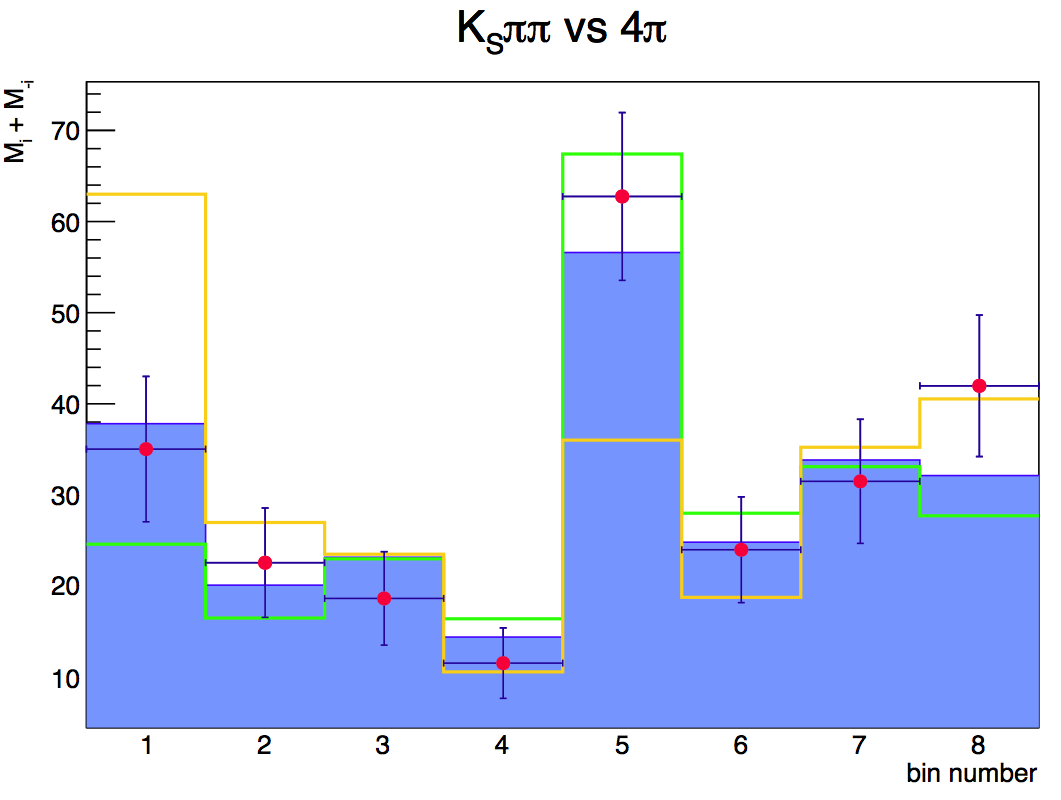
\includegraphics[width=0.48 \textwidth] {KsPiPi_F_Comp.png}}
\subfigure{ 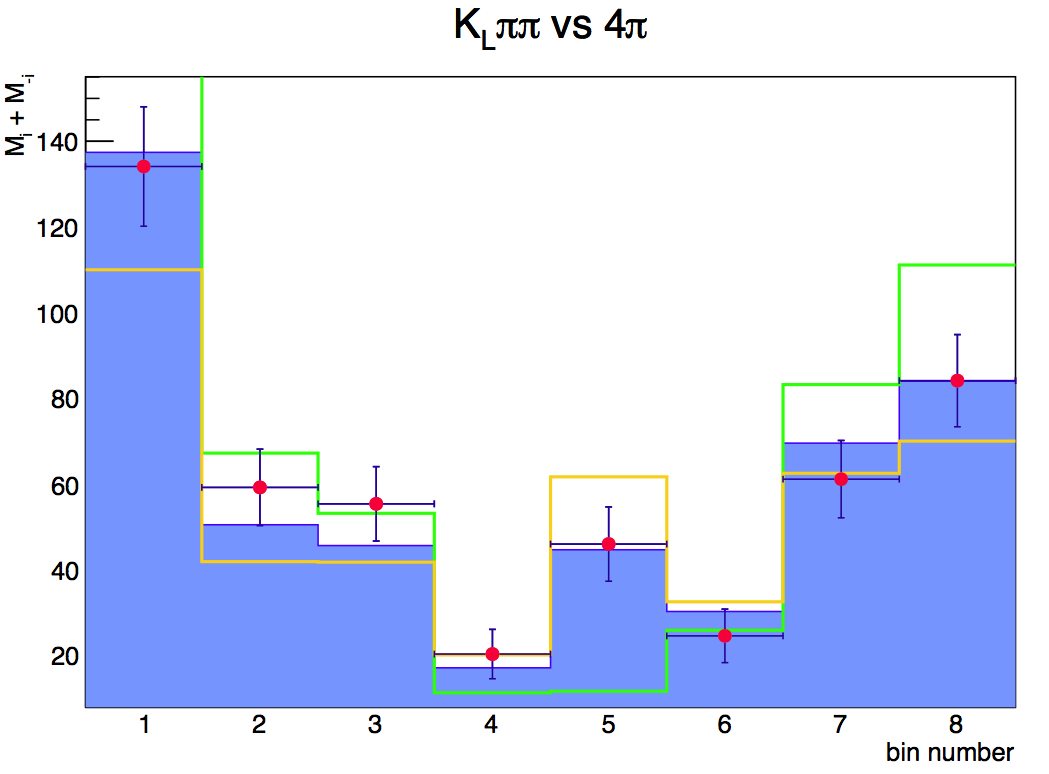
\includegraphics[width=0.48 \textwidth] {KlPiPi_F_Comp.png}}
\end{center}
\caption{\textit{Distribution of signal yields per bin for \KsPiPi (left) and \KlPiPi (right). Red: data, blue histogram: fit results (fit to \KsPiPi and \KlPiPi separately), orange: values for $F_+$=0.5, green: values for $F_+$=1.0.}}
\end{figure}

\begin{figure}[!h]
\begin{center}
 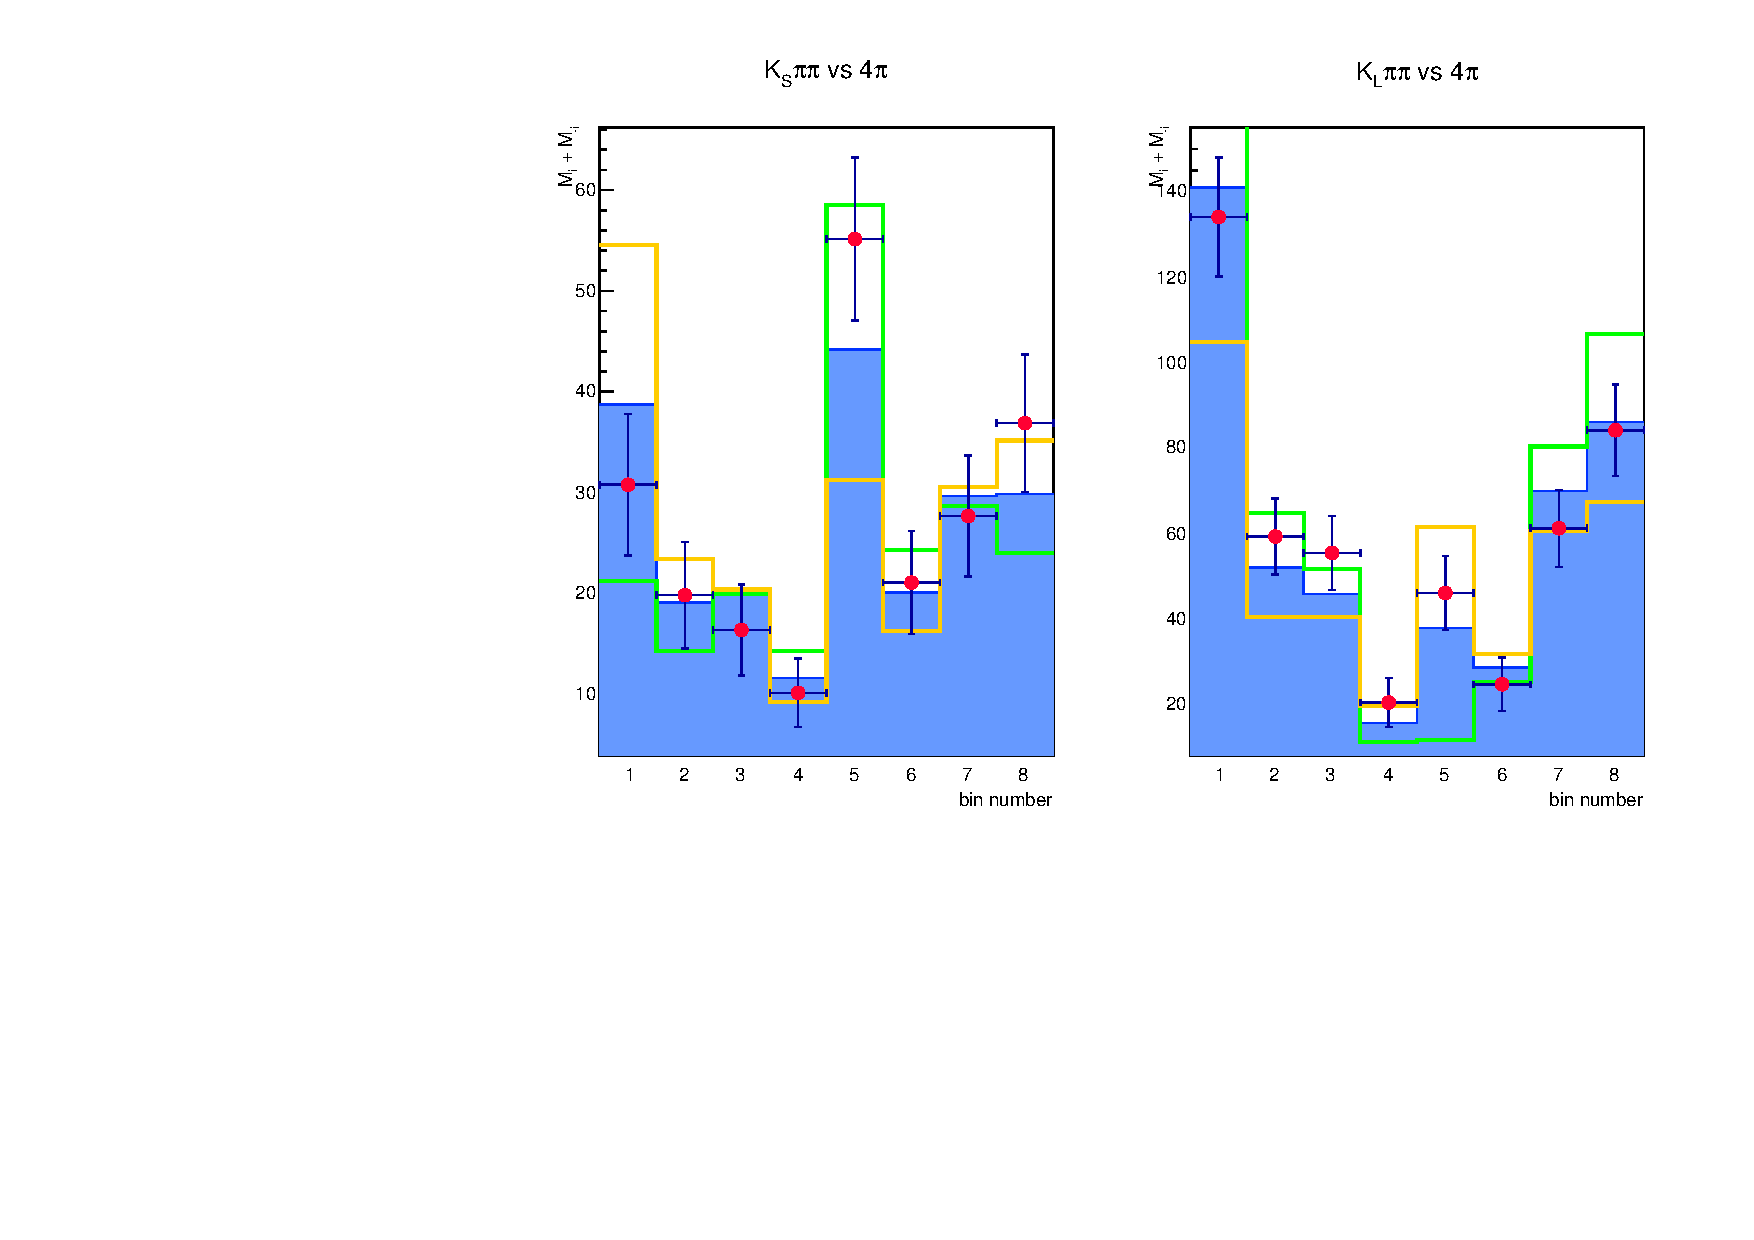
\includegraphics[width=1. \textwidth] {Sim_F_Comp.pdf}
\end{center}
\caption{\textit{Distribution of signal yields per bin for \KsPiPi (left) and \KlPiPi (right). Red: data, blue histogram: fit results (fit to \KsPiPi and \KlPiPi simultaneously), orange: values for $F_+$=0.5, green: values for $F_+$=1.0.}}
\end{figure}